%!TEX program = pdflatex
\let\nofiles\relax
\documentclass[UTF8]{article}
\usepackage{graphicx}
\usepackage{setspace}
% \usepackage{ctex}
\usepackage{indentfirst}
\setlength{\parindent}{2em}  % 用于首行缩进

\usepackage{amsmath}
\usepackage{amsthm} % 使用定理环境
\usepackage{amssymb}
\usepackage{cite}   % 文献
\usepackage[colorlinks,linkcolor=red,anchorcolor=blue,citecolor=green,CJKbookmarks=True]{hyperref}  % 使用链接 但不用默认属性
% CJKbookmarks让链接支持中文
% \usepackage{hyperref}
% \usepackage{geometry}
% \geometry{a4paper,scale=0.8}
\usepackage{algorithm}
\usepackage{algorithmic}
\usepackage{geometry}
\geometry{a4paper,left=2.0cm,right=2.0cm,top=3.0cm,bottom=3.0cm}
\setstretch{1.5}   %  改变行间距
% \newgeometry{left = 2 cm, top= 3 cm}

\title{Instrument price on a specific unbalanced cooperative games:Machine Scheduling Game}
\author{Dis\cdot count}

% \newtheorem{algorithm}{Algorithm}
\newtheorem{thm}{\hspace{2em}Theorem}
\newtheorem{lem}{\hspace{2em}Lemma}
\newtheorem{pf}{\hspace{2em}Proof}
\newtheorem{remark}{\hspace{2em}Remark}
\newtheorem{corollary}{\hspace{2em}Corollary}
%  \newtheorem{def}{Definition}  doesnt work

\begin{document}

\maketitle{}

\section*{Abstract}



Keywords: Cooperative game, scheduling, pricing for coopration.


In this paper, instead of sacrificing the entrepreneur’s profits, we are interested in motivating early investors by reallocating final profits earned from the proposal. Intuitively, we assign more profits to early investors so that their waiting costs are balanced out and the resulting pledging probabilities are raised. Note that more profits allocated to (higher pledging probabilities of) early investors means less profits remain for (lower pledging probabilities of) the late ones. To enhance the overall success rate of a crowdfunding project, it is of utmost importance to provide the entrepreneur with appropriate profit allocation mechanisms. Our main contributions are summarized as follows.
First, to the best of our knowledge, this paper is the first attempt to analytically study the profit
allocation mechanism to enhance the success rates of investment-based crowdfunding projects. Most
literature on crowdfunding, especially investment-based crowdfunding, is empirical and existing efforts
on motivating investors focus on offering additional benefits and price discounts. Our study helps the entrepreneur design an optimal profit allocation mechanism to maximize the success rate without sacrificing the profits of the entrepreneur.
Second, we develop static models to analyze the pledging behavior of investors, and we characterize
the “waiting cost” to explain the inequity between investors at different stages in crowdfunding projects. The main results show that because of the waiting cost, investors who arrive early are less willing to pledge money. It also shows that the entrepreneur should motivate early investors to enhance the success rate of the project. In addition, the extra return given to early investors as an incentive should increase with the waiting cost.
Third, as a generalization, we consider the difference in the number of investors who group as cohorts, arriving at different points in time. We find that investors in different-sized cohorts are not equally sensitive with changes in profit allocation, and the entrepreneur should motivate investors in smaller cohorts to enhance the success rate of his crowdfunding project. This property, together with the effect of the waiting cost, decides the profit allocation strategy of the entrepreneur. In addition, we also provide managerial guidance on how the entrepreneur should adjust the optimal profit allocation mechanism when other factors in the market change.
三方面贡献,首先最重要的 是提出 pricing 的概念, 这个概念不同于已有的 惩罚和补贴; 提出概念之后建立了相应的模型,并且提出了相应的解法,归到一个可以求解的问题; generalization, 对于有权重的部分也可用类似的方法,得到了能这样求解的一般性质;
pricing 对于政府定价有一定的启示.

以及第七的拓展部份 提到 pricing 会有固定的两/三个价格提供稳定

The rest of this paper is structured as follows. The following section reviews relevant literature. We describe the basic problem in Section 3. In Section 4, we analyze the profit allocation mechanism using a
primary model where there are only two potential investors. Section 5 generalizes the results of Section 4 by studying a two-cohort model where there are two cohorts of investors. The conclusions are shown in Section 6.


\section*{Introduction}

At first, we will introduce some preliminary knowledge about cooperative game theory as follows.
A pair $(V,c)$ is usually used to represent a cooperative game with transferable utilities, among which $V=\{1,2,\dots,v\}$ denotes a set of $v$ players and $c:2^{V}\to \mathbb{R}$ indicates the characteristic function of the game. A coalition $s$ is defined as a non-empty subset of players; and $V$ is refered to as the grand coalition containing all the players, $S=2^{V} \setminus\{\emptyset\}$ denotes the set of all feasible coalitions. The characteristic function of the game, $c(s)$, represents the minimum coalitional cost the players in $s$ have to pay in order to cooperate together.
A cost allocation vector $\alpha=[\alpha_{1},\alpha_{2},\dots,\alpha_{v}] \in \mathbb{R}^{v}$ is required by the game to maintain cooperation in the grand coalition, and $\alpha_{k}$ is the cost assigned to players $k \in V$ to assure no individual or group of players has the incentive to deviate. For the convenience of abbreviation, we use $\alpha(s)=\sum_{k\in{s}}\alpha_{k}$ to denote the total cost assigned to the players in coalition $s$.
One of the most important concepts in cooperative game theory is core, which is a cost allocation satisfying two kinds of contraints, one is the budget balance contraint {$\alpha(V)=c(V)$} and the other is the coalitional stability constraints {$\alpha(s) \leq c(s)$}. In other words, core can be expressed as

\[
Core(V,c)= \left\{\alpha:\alpha(V)=c(V), \alpha(s)\leq c(s)\ \text{for all}\ s \in S \setminus\{V\}, \alpha \in \mathbb{R}^{v} \right\}.
\]

When the cost allocation exists, core is called non-empty. And if and only if the core is non-empty, the grand coalition of the associating cooperative game $(V,c)$ will be stable or balanced.

However, cooperative games can be unbalanced in many cases owing to the joint restrictions of the above-mentioned two kinds of constraints. To stabilize the grand coalition in unbalanced cooperative games, researchers have already developed several effective instruments, such as subsidization, penalization and simultaneously subsidization and penalization. The
similarity of these instruments is that there exists an outside party who will take measures to stabilize the grand coalition. But the penalization will always arouse the discontent of players in coalitions, it is promising to find a new instrument to replace the penalization, we call it pricing.
The significant idea of this instrument is that we can erase the role of the third party by collecting pricing as subsidy of the corresponding coalitions.
That being said, the players of the games can stabilize themselves without the third party.

To make the project concrete, we will apply this instrument on the machine scheduling games to show our ideas.


\section{Literature Reviewe}
\cite{caprara2010new}
\cite{liu2018simultaneous}


\section{Motivating problem}

\subsection{Basic concept}

At first, we will introduce some preliminary knowledge about cooperative game theory as follows.
A pair $(V,c)$ is usually used to represent a cooperative game with transferable utilities, among which $V=\{1,2,\dots,v\}$ denotes a set of $v$ players and $c:2^{V}\to \mathbb{R}$ indicates the characteristic function of the game. A coalition $s$ is defined as a non-empty subset of players; and $V$ is refered to as the grand coalition containing all the players, $S=2^{V} \setminus\{\emptyset\}$ denotes the set of all feasible coalitions. The characteristic function of the game, $c(s)$, represents the minimum coalitional cost the players in $s$ have to pay in order to cooperate together.
A cost allocation vector $\alpha=[\alpha_{1},\alpha_{2},\dots,\alpha_{v}] \in \mathbb{R}^{v}$ is required by the game to maintain cooperation in the grand coalition, and $\alpha_{k}$ is the cost assigned to players $k \in V$ to assure no individual or group of players has the incentive to deviate. For the convenience of abbreviation, we use $\alpha(s)=\sum_{k\in{s}}\alpha_{k}$ to denote the total cost assigned to the players in coalition $s$.
One of the most important concepts in cooperative game theory is core, which is a cost allocation satisfying two kinds of contraints, one is the budget balance contraint {$\alpha(V)=c(V)$} and the other is the coalitional stability constraints {$\alpha(s) \leq c(s)$}. In other words, core can be expressed as

\[
Core(V,c)= \left\{\alpha:\alpha(V)=c(V), \alpha(s)\leq c(s)\ \text{for all}\ s \in S \setminus\{V\}, \alpha \in \mathbb{R}^{v} \right\}.
\]

When the cost allocation exists, core is called non-empty. And if and only if the core is non-empty, the grand coalition of the associating cooperative game $(V,c)$ will be stable or balanced.

However, cooperative games can be unbalanced in many cases owing to the joint restrictions of the above-mentioned two kinds of constraints. To stabilize the grand coalition in unbalanced cooperative games, researchers have already developed several effective instruments, such as subsidization, penalization and simultaneously subsidization and penalization. The
similarity of these instruments is that there exists an outside party who will take measures to stabilize the grand coalition. But the penalization will always arouse the discontent of players in coalitions, it is promising to find a new instrument to replace the penalization, we call it pricing.
The significant idea of this instrument is that we can erase the role of the third party by collecting pricing as subsidy of the corresponding coalitions.
That being said, the players of the games can stabilize themselves without the third party.

To make the project concrete, we will apply this instrument on the machine scheduling games to show our ideas.


\subsection{Identical Variable Parallel machine scheduling of Unweighted jobs game}
% 这里还需要定义一个优化问题

The Identical Parallel machine scheduling of Unweighted jobs(IPU) problem can be defined as follows. There are several machines available here. For this scheduling problem, the setup cost for each machine is the same and jobs have the same weights. The problem requires that the jobs should be scheduled to several of these machines in order to have a minimum completion time, which contains the setup costs considered as a form of time and total processing time for all jobs. Thus, we call this problem as the
identical parallel machine scheduling of unweighted jobs problem.
Based on the above scheduling problem we mentioned, we can have the definition of the cooperative game form.
In an Identical Variable Parallel machine scheduling of Unweighted jobs (IVPU) game, each player $k$ in the grand coalition $V=\{1,2,\ldots,v\}$ has a job $k$ that needs to be processed on one of identical machines in $M=\{1,2,\ldots,m\}$, where $m$ is a given positive integer, commonly we set it larger than $v$. Meanwhile, each machine has a setup cost $P$. Each job $k\in V$ has a processing time denoted by $t_k$. Each coalition $s \in S$, where $S=2^V\setminus\{\emptyset\}$, aims to schedule the jobs in $s$ on all machines in $M$ so that the total completion time of the jobs in $s$ is minimized, i.e., to minimize
$c(s,m^*) = \min_{j \in M} \{\sum_{k\in s}{C_k(j)}+ P\cdot j\}$, where $C_k(j)$ is the completion time of job $k\in s$ and it is related to the number of machines used, $m^*$ indicates the optimal number of machines used by the coalition $s$.

Then we will illustrate the pricing instrument with a simple example of an IAPU game as follows.


\subsection{Inspired Example}
There is an IVPU game which contains four players, whose processing times on the identical parallel machine are $t_1=2, t_2=3, t_3=4, t_4=5$ respectively. Each machine setup cost is $t_0=9.5$, and $c(s)$ is the minimum total completion time of jobs in coalition $s$ plus the machine setup costs.
Hence we have the following values of the characteristic functions:

\[
\begin{aligned}
& c({1}) = 11.5, c({2}) = 12.5, c({3}) = 13.5, c({4}) = 14.5  \\
& c({1,2}) = 16.5, c({1,3}) = 17.5, c({1,4}) = 18.5 \\
& c({2,3}) = 19.5, c({2,4}) = 20.5, c({3,4}) = 22.5 \\
& c({1,2,3}) = 25.5, c({1,2,4}) = 26.5, c({1,3,4}) = 28.5 \\
& c({2,3,4}) = 31.5, c({1,2,3,4}) = 38.
\end{aligned}
\]
% $c({1}) = 11.5, c({2}) = 12.5, c({3}) = 13.5, c({4}) = 14.5, c({1,2}) = 16.5, c({1,3}) = 17.5, c({1,4}) = 18.5, c({2,3}) = 19.5, c({2,4}) = 20.5, c({3,4}) = 22.5, c({1,2,3}) = 25.5, c({1,2,4}) = 26.5, c({1,3,4}) = 28.5, c({2,3,4}) = 31.5, c({1,2,3,4}) = 38.$

For the convenience of the following statement, we set the price equal to the setup cost, that is, $P = t_0$.
In this example, the grand coalition has a minimum cost, which is $c(V,m^*) = \min_{m \in M} \{\sum_{k\in V}{C_k(m)}+ P\cdot m\}.$ To show the specific calculation process of $C_k(m)$, we set $m=1$, then $\sum_{k\in V}{C_k(1)} = t_1 + (t_1 + t_2) + (t_1 + t_2 + t_3) + (t_1 + t_2 + t_3 + t_4) + P\cdot 1 =
1 \cdot t_4 + 2\cdot t_3 + 3 \cdot t_2 + 3 \cdot t_2 + 4 \cdot t_1 + P \cdot 1.$
The processing sequence for the jobs is job1 $\to$ job2 $\to$ job3 $\to$ job4 on one machine. When job1 is processing, the rest three jobs have to wait. Therefore, the multiplier before processing time of job1 is $4$. The rest of the above formula can be explained in the same way.
Calculate all cases of the number of machines used, we can obtain that
$c(V,m^*) = \min\{39.5, 38, 44.5, 52\} = 38$ and the optimum number of machine used is $m^* = 2$.
By solving the following LP:
\[
  \mathop{\max}_{\alpha}\{\alpha(V): \alpha(s)\leq c(s),\forall s \in S, \alpha\in\mathbb{R}^{v}\},
\]
we can obtain the optimal allocation is $[6, 8.75, 10.75, 11.75]$.
It's easy to check that the cooperative game in this example is unbalanced because there is no cost allocation satisfying the two kinds of constraints we mentioned above. That means there will be some coalitions deviate from the grand coalition, in order to cooperate at this time, the third party have to take some measures, such as subsidization or penalization in common use.
According to the literature, the subsidy can be calculated by solving the following LP:
\[
  {\omega^*}=\mathop{\min}_{\alpha}\{c(V)-\alpha(V): \alpha(s)\leq c(s)
 ,\forall s \in S, \alpha\in\mathbb{R}^{v}\},
\]
In this case, the subsidy equals $c(V) - \alpha(V) = 0.75$.
When the setup cost increases from 9.5 to 10, that is, the price increment is from 0 to 0.5, two machines are still needed. However, at this time, the grand coalition doesnot need extra subsidy because the price increment($0.5\times 2 =1$) can exactly cover the gap between total cost $c(V)$(39) and the acccepted cost shared among players in the grand coalition $\alpha(V)$(38).

The above discussion raises the question whether it is possible to stabilize a grand coalition not changed from the original global schedule, without any externally-funded subsidy. To have an affirmative answer, we propose a new mechanism referred to as subsidization funded by taxation. Using the example, we can explain this idea as follows. When the external party charges the machine tax at 0.5, which makes the machine activation cost at 10, the global optimal schedule is still to use two machines with a total cost at 39. At the same time, if the third party subsidizes the grand coalition by 1, then the four agents only need to share a cost of 38, and a cost allocation (6, 9, 11, 12) would be acceptable to the agents.

Continue to increase the setup cost from 10 to 11.14, , the number of machine used by the grand coaliton will decrease from 2 to 1, accordingly.

Meanwhile, at this point, the total pricing increment can also just cover the gap between $c(V)$ and $\alpha(V)$ like the above, which means that by using pricing instrument the grand coalition can be stabilized by the players themselves.

Although this case is easily understood, it demonstrates the concept of pricing we have strong interests in. Then we will define the corresponding model to further elaborate on this concept.


%\section{Outline}

For the effective domain $[0, P^*]$, we just need to divide this interval into several parts and the points are denoted as $P_L(V,i), i = 1,2,\ldots,n$.  At first, we don't need to calculate the initial part because this part the corresponding subsidy is 0 always. Then we just need to focus on the latter part which shows some interesting properties we proved above.

For any P in $[0, P^*]$, calculate the subsidy and the corresponding slope (Please refer to Liu et.al.2018) z

Flow path: IPC algorithm, (4q-1)

1-\sum_{s\in S\subset\{V\}} \rho_s

To follow the CP approach(Algorithm 3) to calculate the weak derivative, then use Algorithm 1 to obtain the subsidy \omega(z).

Questions: how to solve the LP(9) and the DP program.


% !TEX root = sum1.tex
\section{Analyses of Model}

\subsection{Model for IVPU game}

A cooperative TU game $(V,c)$ is called an IVPU game if the characteristic function satisfies the following formulations.

\[
\begin{aligned}
c(s,P) = & {\min} \sum_{k\in V}\sum_{j\in O} {c_{kj} x_{kj}} + {P\sum_{k\in s} x_{k1}} \\
{s.t.}\quad & \sum_{j \in O} x_{kj}-y_k^s=0, \forall k \in V, \\
& \sum_{k\in V} x_{kj} \leq m,\forall j \in O,  \\
& x_{kj} \in \{0,1\} , \forall k \in V, \forall j \in O,\\
& y_k^s=1, k \in s, y_k^s=0, k \notin s.
\end{aligned}
\]

The first set of constraints indicate that only jobs in $s$ are included and are processed only once.
Notice that $ y_k^s=1, k \in s$, the constraints are equivalent to $\sum_{j \in O} x_{kj}-1=0, k \in s$.
The second set of constrains indicate that at most $m$
machines can be used, and they assure that no jobs are processed on the same machines at the same time.

Among these formulations, $P$ and $m$ denotes the price and maximum number of machines available, respectively. Note that $j$ represents the processing sequence on the machines, so when $j=1$, $\sum_{k\in s} x_{k1}$ indicates all machines used by coalition $s$, i.e., the optimal machine number.

To be consistent with the above definition of the grand coalition, let $V=\{1,2,\ldots,v\}$ be a set of $v$ players. The setup cost or price(We will use the term in the remainder of this article.) for each machine is $P$.

% For the convenience of expression, we set the processing times $t_i(i\in V)$ satisfy $t_1<t_2<\cdots<t_v$.

Then we need to define two functions, practical subsidy-price function (PSPF) and theoretical subsidy-price function (TSPF) denoted by $\omega(P)$ and $\hat{\omega}(P)$, respectively:
\[
  {\omega(P)}=\mathop{\min}_{\alpha}\{c(V,P)-\alpha(V): \alpha(s) \leq c(s,P)
 ,\forall s \in S, \alpha\in\mathbb{R}^{v}\},
\]
\[
  {\hat{\omega}(P)}=\mathop{\min}_{\alpha}\{c(V,P)-\alpha(V): \alpha(s) \leq c(s,P)
 ,\forall s \in S\setminus\{V\}, \alpha\in\mathbb{R}^{v}\}.
\]
PSPF has one more inequality $\alpha(V)\leq c(V,P)$ than TSPF, which ensures the minimum value of PSPF is 0, while TSPF can have a negative value. PSPF is our top priority because we think the value of subsidy is positive commonly. However, TSPF can also provide us with a theoretical perspective.

Then we need to define an interval $[P_L(i,V),P_H(i,V)]$ to denote the price range when the grand coalition $V$ uses $i$ machines to obtain the minimum cost for scheduling jobs. And the effective domain of pricing IVPU game for stabilization is $[0,P^*]$.
In other words, the price should have practical significance, that is, the negative price is beyond of our consideration in this situation. Thus, the minimum price for each machine is 0. Meanwhile, the maximum price for each machine will be infinity in theory, later we will show a more meaningful price instead of $P^*$ defined here.

Based on the above analysis, we know that $c(s,P) = \min_{i \in M} \{\sum_{k\in s}{C_k(i)}+ P\cdot i\}.$ Define a no-price characteristic function $c_0(s,i)$
related to the number of machines $i \in \{1,2,\ldots,v\}$ used by coalition $s.$ Meanwhile, $c_0(V,i)$ denotes the cost of using $i$ machines by the grand coalition and it is determined by $i$ when the processing time of every player in the grand coalition is known.
Therefore, the original characteristic function can be expressed in two parts like $c(s,P) = c_0(s,m^*) + P\cdot m^*$, where $m^*$ is the optimal number of machines used by coalition $s$.

We set the different intervals where the number of machines remain unchanged as $I_i$ respectively.
Assume that the optimal schedule is that the grand coalition uses $i$ machines, the price for each machine is $P^i$ which belongs to the interval $I_i$.
Then according to the definition of the characteristic function, we can obtain the following two inequalities:
\[
\begin{aligned}
&c_0 (V,i) + P^i i \leq c_0 (V,i-1) + P^i\cdot(i-1) \\
&c_0 (V,i) + P^i i \leq c_0 (V,i+1) + P^i\cdot(i+1).
\end{aligned}
\]
Consequently, we obtained the range of the price $P^i$ satisfies $c_0 (V,i) - c_0 (V,i+1) \leq P^i \leq c_0 (V,i-1) - c_0 (V,i)$.
That is to say, $P^i$ at least belongs to interval $[c_0 (V,i) - c_0 (V,i+1), c_0 (V,i-1) - c_0 (V,i)].$
We will continue to investigate the relationship between this interval and the above mentioned $I_i$.

% If we assume that the processing times satisfy $t_1 < t_2 < \ldots < t_v$, then $c_0(V,i) = \sum_{j=1}^{\lceil v/i \rceil} \sum_{h=1}^i j t_{v-ij-h+i+1}$, where $\lceil \cdot \rceil$ is the minimum integer larger than $\cdot$.

If we assume that the processing times satisfy $t_1 > t_2 > \ldots > t_v$, then $c_0(V,i) = \sum_{k=1}^{v} {\lceil k/i \rceil} t_{k}$, where $\lceil \cdot \rceil$ is the minimum integer larger than $\cdot$.

According to $c_0(V,i) = \sum_{k=1}^{v} {\lceil k/i \rceil} t_{k}$, it is easy to know that the multipliers of all the processing times $t_k, k \in V$ decrease correspondingly with the increase of the number of machines used.

Besides that, we can also prove that $\sum_{k=1}^{v} ({\lceil k/i \rceil} - {\lceil k/(i+1) \rceil}) t_k < \sum_{k=1}^{v} ({\lceil k/(i-1) \rceil} - {\lceil k/i \rceil}) t_k.$

Proof tips: Let $p_i(k)$ denote ${\lceil k/i \rceil}$, the $k$th multipliers of $t_k$. At first, $p_{i-1}(i)- p_i(i)=0 ~\text{or}~ 1$. Then the multiplier difference of $t_i$ is $p_{i-1}(i)- p_i(i)=1$, while $p_i(i) - p_{i+1}(i)=0$
Meanwhile, the multiplier difference of $t_{i+1}$ is $p_{i-1}(i+1)- p_i(i+1)=0$ and $p_i(i+1) - p_{i+1}(i+1)=1$. However, because of $t_{i} > t_{i+1}$, put the two numbers together we can get $(p_{i-1}(i)- p_i(i))t_i + (p_{i-1}(i+1)- p_i(i+1))t_{i+1} > (p_{i}(i)- p_{i+1}(i))t_i + (p_{i}(i+1)- p_i(i+1))t_{i+1}$.
The above relationship holds when the ordinal number $k$ satisfies $k = (l-1)i, l = \{2,3,\ldots,i\}$.
When $k > (i-1)i$, $p_{i-1}(k)- p_i(k) \geq p_{i}(k)- p_{i+1}(k)$. And when for other cases, it is easy to prove $p_{i-1}(k)- p_i(k) \geq p_{i}(k)- p_{i+1}(k)$.

So we have the following theorem:
\begin{thm}\label{monotone}
For the IVPU game, the no-price characteristic function $c_0(V,i)$ is monotone decreasing and concave with $i$, in other words, $c_0(V,i)$ satisfies the following inequalities:
\[
\begin{aligned}
& c_0(V,i)- c_0(V,i-1) < 0, i \in \{2,3,\ldots,v\}\\
& c_0 (V,i) - c_0 (V,i+1) < c_0 (V,i-1) - c_0 (V,i), i \in \{2,3,\ldots,v-1\}.
\end{aligned}
\]
\end{thm}

In the light of the Theorem \ref{monotone}, $c_0(V,i)- c_0(V,i-1) < 0$ ensures that the value of price is positive. Moreover, $c_0(V,i)$ is concave with $i$,  the interval will not be empty and $I_i = [c_0 (V,i) - c_0 (V,i+1), c_0 (V,i-1) - c_0 (V,i)], i \in \{2,3,\ldots,v-1\}.$ Define $I_1 = [c_0 (V,1) - c_0 (V,2), P^*]$ and $I_v = [0, c_0 (V,v-1) - c_0 (V,v)]$, until here, the effective domain $[0, P^*]$
is divided into $v$ non-overlapping sub-intervals $I_i, i\in V$.

\begin{remark}
  Denote the left and right extreme points of the interval $I_i$ as $P_L(i,V), P_H(i,V)$ respectively. It's easy to know that $P_L(i,V) = P_H(i+1,V)$.
\end{remark}

\begin{remark}
  Note that $P_L(i,V) = P_H(i+1,V)$, for the sake of brevity and readability, we use $P_{i+1}$ to substitute for $P_L(i,V)$ or $P_H(i+1,V)$ later on.
\end{remark}

\begin{remark}
  For ease of exposition, let $P_1 = P^*, P_L(v,V) = 0$ and $P_i = P_H(i,V) = P_L(i-1,V), i \in \{2,3,\ldots,v\}.$ Thus, the effective domain, $[0,P^*]$, is divided into $v$ non-overlapping sub-intervals by $P_i, \forall i \in \{2,3,\ldots,v\}$.
\end{remark}

\begin{remark}
  $P^*$ is the lowest price under which the grand cooperation of IVPU game is stable and it uses only one machine in the optimal scheduling decision, i.e.,
  $P^* \in (P_L(1,V), P_H(1,V)]$ and MSG$(V, c(\cdot, P^*))$ has non-empty core.
\end{remark}


\subsection{Properties of IVPU game}
Like the above, divide the characteristic function into two parts like $c(s,P) = c_0(s,m^*(s)) + P\cdot m^*(s), s \in S$.

As a common practice, we can obtain the dual of $\omega(P)$:
\begin{equation}\label{dual}
 {\omega^*(P)}=\mathop{\max}_{\rho} \{c_0(V, m^*(V))+ m^*(V)P + \sum_{s\in S}-\rho_s[c_0(s,m^*(s)) + P\cdot m^*(s)]:
 \sum_{s\in S:k\in s}\rho_s=1,\forall k \in V,\rho_s\geq 0,\forall s \in S \}
\end{equation}

By deriving $\omega^*(P)$ with respect to $P$, we can obtain lemma \ref{sum_slope}.

\begin{lem}\label{sum_slope}
The sum of absolute values of slopes at both sides of $P_i$ is 1.
\end{lem}

Based on the above defined PSPF, we can establish Theorem \ref{piecewise} below, showing the property of this function.

\begin{thm}\label{piecewise}
$\omega(P)$ is piecewise linear, and convex in price P at each sub-interval $[P_{i+1},P_{i}], i \in \{1,2,\ldots,v-1\}$.
\end{thm}

In this situation, the size of interval $I_i$ can be calculated when $t_i,i \in \{1,2,\ldots,v\}$ is known. As shown previously, the extreme points of these intervals are recorded as $P_i$ respectively, which represents the price when the number of using machine changes from $i$ to $i-1$. Specially, $P_1$ denotes the right extreme point of the whole interval, which is the value of price when using one machine and subsidy equals zero.

Note that the costs of all the exponential coalitions can be easily calculated by the SPT rules, we have lemma \ref{break_price}.

\begin{lem}\label{break_price}
The breaking price, $P_i(2 \leq i \leq v)$, which is at the extreme points of the sub-intervals $I_i$ can be obtained by SPT rules in polynomial time.
\end{lem}

According to the above lemma \ref{break_price}, we can obtain all the extreme points of the sub-intervals $P_i, 2 \leq i \leq v$. When the price increase from $P_i^-$(little smaller than $P_i$) to $P_i^+$(little larger than $P_i$), the number of machines used by the grand coalition will decrease one.

\begin{thm}\label{boundary_price}
Boundary price $P^*$ or $P_1$ equals $\sum_{i=2}^v P_i$, and can be obtained in polynomial time.
\end{thm}

With theorem \ref{boundary_price}, we obtain all the breakpoints during the whole price interval $[0,P^*]$. Then we'll focus on the specific property of subsidy.

\begin{thm}\label{zero_subsidy}
$\omega(P)$ can be bounded by zero when the number of machines used by the grand coalition $V$ is larger than $\frac{v}{2}$.
\end{thm}

In other words, when the number of machines used is larger than half of players, the grand coalition doesnot need any subsidy from the externality.

Define a new game, that is Single Machine Scheduling Game(SMSG)
\[
\begin{aligned}
c(s,P,'m='1) = & {\min} \sum_{k\in V}\sum_{j\in O} {c_{kj} x_{kj} + P} \\
{s.t.}\quad & \sum_{j \in O} x_{kj}-y_k^s=0, \forall k \in V, \\
& \sum_{k\in V} x_{kj} \leq 1, \forall j \in O,  \\
& x_{kj} \in \{0,1\} , \forall k \in V, \forall j \in O,\\
& y_k^s=1, k \in s, y_k^s=0, k \notin s.
\end{aligned}
\]

\begin{thm}\label{SMSG}
For SMSG(or, MSG with only one machine), given $P \in [P_2, P^*]$ (or, $[P_2,P_1]$),
the slope range of each segments in the interval for function $\omega(P)$ is within $\left(-1, -\frac{1}{n-1} \right]$, and the number of breakpoints in the same interval for function $\omega(P)$ is within $O(v^2)$.
\end{thm}

Until here, we described the main property of the whole figure.
And a diagram of the number of machines used and subsidy on price with essential features is showed below.

% \begin{figure}[h] %图
% 	\centering  %插入的图片居中表示
% 	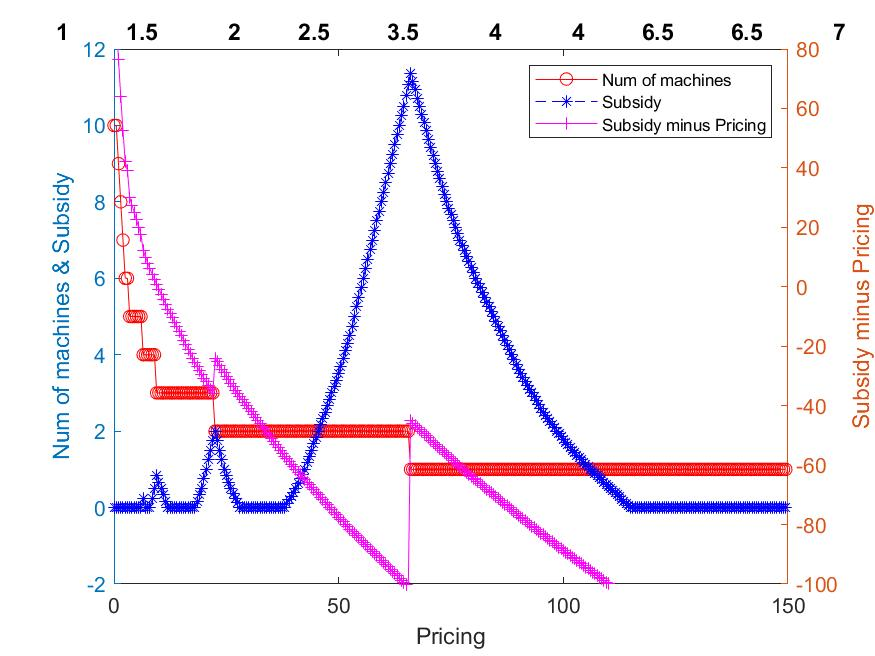
\includegraphics[width=0.8\linewidth]{Figures/Image1}  %插入的图,包括JPG,PNG,PDF,EPS等,放在源文件目录下
% 	\caption{The number of machines and subsidy on setup cost.}  %图片的名称
% 	\label{fig:Image11}   %标签,用作引用
% \end{figure}

As a constrast, we plot the figure of TSPF as below. The difference between practical subsidy-price function (PSPF) and theoretical subsidy-price function (TSPF) is only showed in the inverval when price is larger than $P_1$. This phenomenon matches the Theorem \ref{zero_subsidy}.

% \begin{figure}[h]%图
% 	\centering  %插入的图片居中表示
% 	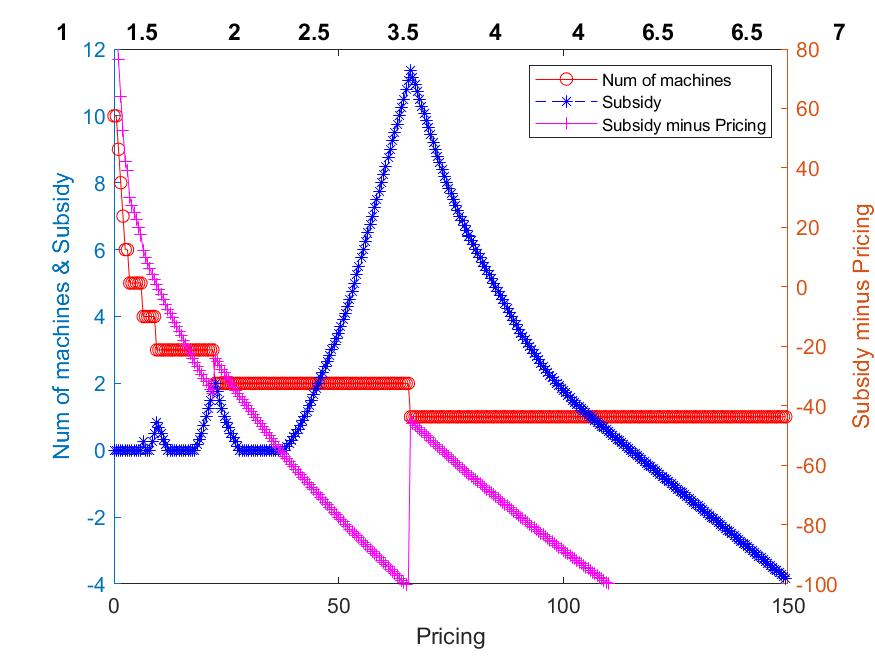
\includegraphics[width=0.8\linewidth]{Figures/Image2}  %插入的图,包括JPG,PNG,PDF,EPS等,放在源文件目录下
% 	\caption{The number of machines and subsidy on setup cost.}  %图片的名称
% 	\label{fig:Image11}   %标签,用作引用
% \end{figure}


\begin{figure}
\begin{minipage}[t]{0.5\linewidth}
\centering
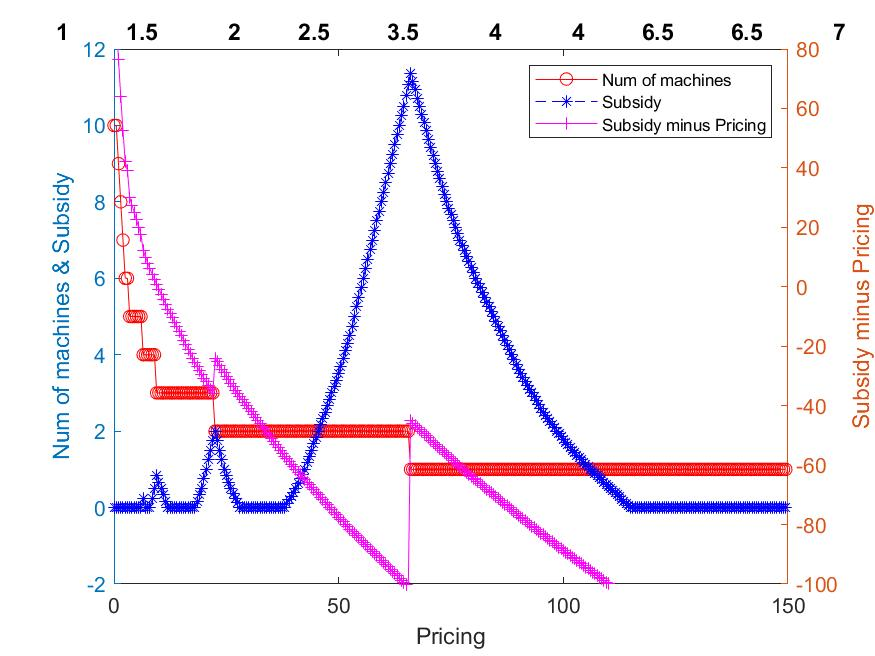
\includegraphics[width=3in]{Figures/Image1}
\caption{PSPF function on pricing}
\label{fig-PSPF}
\end{minipage}%
\begin{minipage}[t]{0.5\linewidth}
\centering
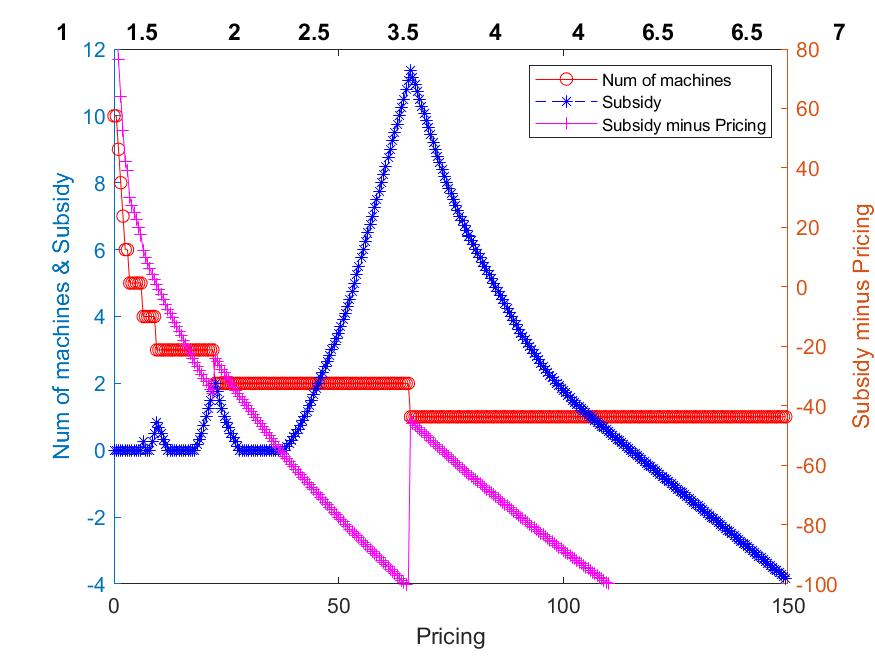
\includegraphics[width=3in]{Figures/Image2}
\caption{TSPF function on pricing}
\label{fig-TSPF}
\end{minipage}
\end{figure}


\begin{remark}
  When the number of available machines $m$ is larger than $v$, the image is complete, just like the above shown. However, when the number of available machines $m$ is less than $v$, the image will be truncated, which means the corresponding part of the price less than $P_{m+1}$ should be removed from the figure. While the properties of the rest part will still hold.
\end{remark}

The processing times of all jobs with the arrangement from small to large are listed on the top of this figure.
The red and blue lines stand for the machine number and subsidy, respectively.
The horizontal ordinate represents the price.
The left ordinate represents the number of machine used, while the right represents the value of subsidy.

Compared with the traditional characteristic function $c(s)$, characteristic function defined in the IVPU game has another parameter, the number of machines used by coalition $m(s)$, whose exponential numbers of $m(s)$ bring more difficulties to the solution.
In order to address this problem, we establish the Theorem \ref{w1P}.

\begin{thm}\label{w1P}
  Define that
  \[
    {\omega_1(P)}=\mathop{\min}_{\alpha}\{c(V,P)-\alpha(V): \alpha(s)\leq c(s,P,1), \forall s \in S, \alpha\in\mathbb{R}^{v}\},
  \]
then the original problem $\omega(P)$ is equivalent to $\omega_1(P)$.
\end{thm}

As the coalitional stability constraints showed above, the exponential inequality constraints are so tricky that we must figure out a method to eliminate redundant constraints to obtain the optimal results.

With the Theorem \ref{w1P}, which will save us from the trouble of solving $c(s, P)$ and speed up the solution, we can use the cutting plane method to eliminate the redundant inequalitie, then  any value of $\omega_1(P)$ can be polynomially solvable when given $P$.


\section{Algorithms for solving IVPU game}
To construct the whole diagram of $\omega(P)$ in $[0,P^*]$, we need to obtain the specific subsidy value $\omega(P)$ given any $P$, which is piecewise linear and convex at every sub-interval. As long as we find all breakpoints during the interval, to get the whole diagram we just need to connect these breakpoints in order.

At first, we need to divide the interval into $v$ sub-intervals according to the number of machines used by the grand coalition. However, we don't need to calculate the interval $[0,P_{\lceil v+1/2 \rceil}]$ because at this part the corresponding subsidy is 0 always.(The corresponding conclusion we mentioned in Theorem \ref{thm4})
Then we just need to apply the IPC algorithm on the rest interval to get the breakpoints. After obtaining all the breakpoints, the PSPF function can be constructed.

\subsection{IPC Algorithm}

\begin{algorithm}[h]\label{algoIPC}
\caption{The Intersection Points Computation(IPC) Algorithm to Construct the PSPF Function.}
\begin{algorithmic}[1]

\begin{description}
  \justifying
  \item[Step 1.] Initially, set $I^*=\{P_L,P_H\}$ and $\mathbb{I}= \{[P_L,P_H]\}$.
  \item[Step 2.] If $\mathbb{I}$ is not empty, update $I^*$ and $\mathbb{I}$ by the following steps:
  \item[Step 3.] Sort values in $I^*$ by $P_0<P_1<\cdots<P_q$, where $P_0 = P_L,P_q = P_H$ and $q = |I^*|-1$.
  \item[Step 4.]
  Select any interval from $\mathbb{I}$, denoted by $[P_{k-1},P_{k}]$ with $1\leq k \leq q$
  \item[Step 5.]
  Construct two linear function $ R_{k-1}(P)$ and $ L_{k}(P)$ so that $ R_{k-1}(P)$ passes $(P_{k-1},\omega(P_{k-1}))$ with \\
  \vspace{10pt}
  a slope equal to a right derivative $K_{r}^{P_{k-1}}$ of $\omega(P)$ at $P_{k-1}$, and that $L_{k}(P)$ passes $(P_{k},\omega(P_{k}))$ with a \\
  \vspace{10pt}
  slope equal to a left derivative $K_{l}^{P_{k}}$
  of $\omega(P)$ at $P_k$.
  \item[Step 6.] If $R_{k-1}(P)$ passes $(P_{k},\omega(P_{k}))$ or $L_{k}(P)$ passes $(P_{k-1},\omega(P_{k-1}))$, then update $\mathbb{I}$ by removing \\

  $[P_{k-1},P_{k}]$. Otherwise, $R_{k-1}(P)$ and $L_{k}(P)$ must have a unique intersection point at $P=P'$ for  \\
  \vspace{10pt}
  some $P' \in (P_{k-1},P_{k})$.
  Update $I^*$ by adding $P^'$, and update $\mathbb{I}$ by removing $[P_{k-1},P_{k}]$, adding \\
  \vspace{10pt}
  $[P_l,P']$ and $[P',P_r]$.
  \item[Step 7.] Go to step 2.
  \item[Step 8.] Return a piecewise linear function by connecting points $(P,\omega(P))$ for all $P \in I^*$.

\end{description}
\end{algorithmic}
\end{algorithm}

\begin{figure}[h]%%图
	\centering  %插入的图片居中表示
	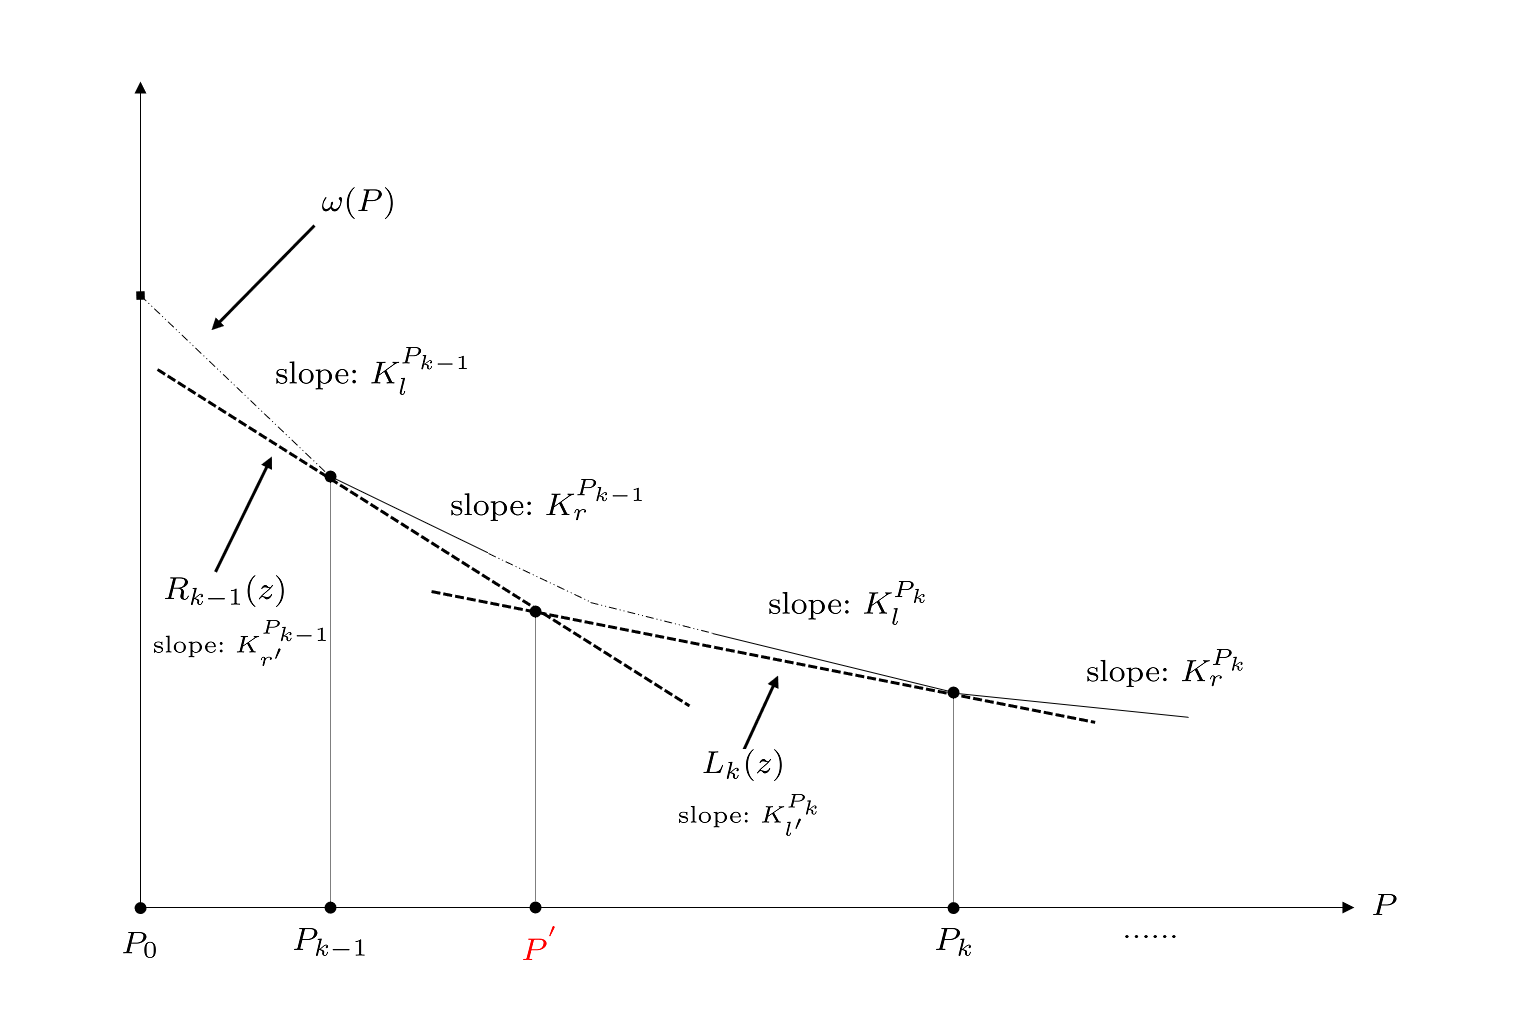
\includegraphics[width=0.9\linewidth]{Figures/IPC}
	\caption{The effects of IPC algorithm applying on the sub-interval.}  %图片的名称
	\label{fig:ImageIPC}   %标签,用作引用
\end{figure}

Then we need to calculate the $\omega(P)$ when given an arbitrary $P$. As stated previously, the value of $\omega(P)$ equals to $\omega_1(P)$. The latter one in fact is a form of simultaneously penalization and subsidization mentioned by Liu et.al.2018.

Then we can follow the basic Cutting Plane(CP) algorithm to solve the tricky exponential inequality constraints $\alpha(s) \leq c_0(s,1)+P$, the specific process are represented in algorithm 2.

\subsection{CP Algorithm}

\begin{algorithm}[h]\label{algoCP}
\caption{The Cutting Plane(CP) Algorithm to compute $\omega(P)$ for a given $P$.}
\begin{algorithmic}[1]

\begin{description}
  \justifying
  \item[Step 1.] Let $\mathbb{S}'\subseteq \mathbb{S}\setminus \{V\}$ indicates a restricted coalition set, which includes some initial coalitions,
  \vspace{10pt}
  e.g.,$ \{1\},\{2\},\ldots,\{v\}$.
  \item[Step 2.] Find an optimal solution $\bar{\alpha}(\ \cdot \ ,P)$ to LP $\tau(P)$:
  \begin{equation*}
  \max_{\alpha\in \mathbb{R}^v} \big\{ \alpha(V,P): \alpha(s,P) \leq c_0(s,1)+P, \mbox{ for all } s \in \mathbb{S}'\big\}.
  \end{equation*}
  \vspace{-11pt}
  \item[Step 3.]
  Find an optimal solution $s^*$ to the separation problem:
  \begin{equation*}
  \delta = \min \big\{ c_0(s,1)+ P -\bar{\alpha}(s,P): \forall s \in \mathbb{S} \setminus \{V\}\big\}.
  \end{equation*}
  \item[Step 4.]
  If $\delta<0$, then add $s^*$ to $\mathbb{S}'$, and go to step 2; otherwise, return $\omega(P)=c(V,P)-\bar{\alpha}(V,P)$ and the pair of derivatives $(K_{l}^{\bar{\beta}},K_{r}^{\bar{\beta}})$.
\end{description}

\end{algorithmic}
\end{algorithm}

As we all know, the cost arised from the partial players in the grand coalition, that is $c(s,P)$, can be calculated handily by the SPT rule (The corresponding conclusion see Lemma \ref{lem1}).
Now, the question is how to solve the separation problem mentioned above efficiently.

\begin{lem}\label{lem3}
  For the AIPU game, the corresponding separation problem can be sovled in $O(v^2)$ time, which could be shown in the following DP algorithm.
\end{lem}

Assume that the processing jobs satisfy $t_1 \geq t_2 \geq \ldots \geq t_v$. For the separation problem $\delta_{AIPU} = \min \big\{ C'(S,P) -\bar{\alpha}(S,P): \forall S \in \mathbb{S} \setminus \{V\}\big\}$, where $C'(S,P)$ can be obtained by the SPT rule. That means if add a new player $k\notin S$ into $S$, where $|S| =u$, the increment for the restricted separation problem is $(u+1)t_k-\alpha_k$, which will be shown in the recursion in \textbf{Step 3}.

\subsection{DP Algorithm}

\begin{algorithm}[h]\label{algoDP}
\caption{The Dynamic Programming(DP) Algorithm to Solve the seperation problem.}
\begin{algorithmic}[1]

% the coalition $s$ is a subset of $\{1,2,\ldots,k\}$.
\begin{description}
  \item[Step 1.] Initially, let $D(k,u)$ indicate the minimum objective value of the restricted problem of separation \\
  \vspace{10pt}
  problem $\delta_{AIPU}$, where $k$ is a player in the grand coalition and $u$ is the number of players included in $S$. So $ k \in \{1,2,\ldots,v\}$ and $u\in \{0,1,\ldots,v\}$.

  \item[Step 2.] Given the initial conditions $D(1,0) = P$ and $D(1,1) = t_1 - \beta_1 +P$. The boundary conditions are \\
  \vspace{10pt}
  $D(k,u) = \infty$ if $u > k$, for all $k \in V$.
  \item[Step 3.] Given the recursion:
  \begin{equation*}
  D(k,u)= \min \left\{
  \begin{aligned}
  & D(k-1,u), \text{for the case when} \ s^* \ \text{does not contain} \ k, \\
  & D(k-1,u-1) + u t_k - \alpha_k ,\text{for the case when} \ s^* \ \text{contains} \ k.
  \end{aligned}
  \right.
  \end{equation*}

  \item[Step 4.] Obtain the optimal objective value of separation problem by
  $\delta_{IVPU} = \min\{D(v,u): u\in \{1,2,\ldots,v-1\}\}$.
   return $\delta_{AIPU}$.
\end{description}

\end{algorithmic}
\end{algorithm}

{The DP Algorithm can solve the separation problem $\delta_{AIPU}$ in $O(v^2)$ time.}
Notice that $k \in \{1,2,\ldots,v\}$ and $u\in \{0,1,\ldots,v\}$ for the $D(k,u)$, so the total running time is in $O(v^2)$.

Now we know the separation problem can be solved in $O(v^2)$ time and the breakpoints during the whole interval are polynomial, so for the IVPU game the PSPF function can be constructed in polynomial time.

\begin{thm}\label{thm6}
The IVPU game can be solved in polynomial time.
\end{thm}

Until here, we've solved the IVPU game with alternative machines.


% !TEX root = sum1.tex
\section{Game Extension}
 % 提到 pricing 会有固定的两/三个价格提供稳定  不存在 机器数量不变/scheduling的情况下, 可以稳定.
% 把 理论的补贴函数画一下,做下比较,不是重点,但要说明
% 把证明没写的补充一下.

Most analyses are applicable to the Machine Scheduling Game with Weighted jobs(MSGW).
In this game, each job $k \in V$ has a processing time, $t_k$, and a weight, $w_k$.
Note that the properties of this game is similar to the unweighted one, we will show main properties briefly in the following.

\begin{corollary} \label{cor-1}
$c(s,P)$ and $P_i(2 \leq i \leq v)$ can be obtained by analysing the order of $t_k/\omega_k$ instead of $t_k$.

\end{corollary}

\begin{corollary} \label{cor-2}
  $\omega(P)$ is piecewise linear, convex in price $P$ at each subinterval.
\end{corollary}

\begin{corollary} \label{cor-3}
  IPC, CP algorithms can be used to construct function $\omega(P)$ in polynomial time.
\end{corollary}

The notations, such as $c(s,P), \omega(P), P_i$ are the same as the above defined.

\begin{lem}\label{lem4}
When $c_0(s)$ satisfy the supermodular and $P=P_1$, where $m_V=1$, if $\alpha(s)=c(s, P_1), \left| s \right|= n-1$ and $\alpha(V)=c_0(V)+P_1$ the budget balance constraint holds, the other coalitional stability constraints $\alpha(s) \leq c(s, P_1) \left| s \right| < n-1$ will hold.
\end{lem}

As we've already known that $P_i, i = 2,\ldots,n$ can be obtained by Lemma \ref{lem1} and Theorem \ref{thm2}, however, $P_1$ can be calculated by solving the $n$ equalities by Lemma \ref{lem4}.

Then we can follow the CP approach (Algorithm 3 in Liu et.al.2018) to calculate the weak derivatives at each sub-interval $[P_L(m,V),P_H(m,V)]$ where the corresponding derivative is $m_V-\sum_{s\in S\setminus\{V\}} \rho_s$.

Then use IPC Algorithm which will return all the breakpoints during the $[0, P^*]$ to obtain the subsidy $\omega(P)$.

Notice that we can calculate the characteristic function $c(s)$ easily according to Theorem \ref{thm5}, we can formulate Theorem \ref{thm6}.


Remind that we want to realize that a situation that don't need a subsidy from the externality.
It gives the method to determine the price

By minusing the increment part, we can get a monotone decreasing line in every sub-interval, so doesnot exist the situation where we do not need change the original schedule to stabilize the grand coalition.

And whether exist one point or two or three, it depends on the the relationship of $P_1,P_2, P_3$.
which depends on the value of the processing time. When the processing time is close to each other, we can conclude that the there exists two points to satisfy the requirement.

There only exist at most three price to choose, and commonly two depends on the processing time.


Then, we will try to extend the core concept to a more general case. So we need to define a new game as follow.

\subsection*{General model}

A cooperative TU game $(V,c)$ is a PIM(Price Integer Minimization) game if there exist:

\begin{itemize}
	\item positive integers e, v, t, P and m;
	\item integer vectors $ x \in \mathbb{Z}^{t \times 1} $and $ \tilde{\alpha} \in \mathbb{Z}^{1 \times t} $;
	\item left hand side matrix  $A \in \mathbb{R} ^{e \times t};$
	\item right hand side matrix $B \in \mathbb{R} ^ {e \times v};$
	\item a right hand side vector $D \in \mathbb{Z} ^ {e};$
	\item an objective function vector
	$c \in \mathbb{Z}^{1 \times t};$
	\item an incidence vector $y^s \in \{0,1\}^v$ with $y^s_k = 1$ if $k \in s$ and $y^s_k = 0 $ otherwise, $\forall k \in V$,

\end{itemize}

such that the characteristic function $c(s)$ equals the optimal objective value of the following integer linear program:

\[
c(s,P)= \mathop{\min}_{x} \{ cx+Pm(x): Ax \geq By^s+D, \tilde{\alpha}x \leq m, x \in \mathbb{Z}^{t \times 1} \}
\]

Note that the object function is not easy to analyze due to the joint effct of $cx$ and $Pm$, we need to divide the function into two parts for a further discussion.

With this idea, we divide $c(s,m(s,P))$ as $c_0(s,m(s))+Pm $. Via analysis and study, we find some properties about $c_0(s,m(s)) $ which we call primary function later.

The primary function must be supermodular, then we can get the positive price or setup cost when the number of facilities changes. This corresponds to the following two lemmas.


\begin{lem}\label{lem2}
% \\ \hspace*{\fill} \\ % 用于空行
% ~\\
\[c_0(V,m)- c_0(V,m-1) > 0 \Leftrightarrow P_m > 0, m=2,\ldots,n.\]
\end{lem}

\begin{lem}\label{lem3}
\[
\begin{aligned}
&c_0 (V,m) - c_0 (V,m+1) < c_0 (V,m-1) - c_0 (V,m) \\
&\Leftrightarrow \quad P_m < P_{m+1} , m=2,3,\ldots,n.
\end{aligned}
\]
\end{lem}

Once the primary function must be supermodular, we can specify this property in the following two aspects.
One is the concavity about the number of facilities,
the other is the nature about the number of players($s_1 \subset s_2$).
They correspond to the following two formulas:

\begin{equation}\label{concavity_f}
c_0(s_1,m-1)-c_0(s_1,m) \geq
  c_0(s_1,m)-c_0(s_1,m+1) \quad m=2,\ldots,n.
\end{equation}
% 只要这里是关于机器数量的变化即可
and

\begin{equation}\label{property_p}
	c_0(s_1,m-1)-c_0(s_1,m) \leq
	  c_0(s_2,m-1)-c_0(s_2,m) \quad m=2,\ldots,n.
\end{equation}
, respectively.
% 只要这里是关于 players 的变化即可

If the characteristic function satisfies the above property. Then $ P_1$ can be calculated by the following procedure:
When $\alpha(V) = c_0(V) + P_1$, which means the $\omega(P_1) = 0$. And the active inequalities must be the coalition contains $(n-1)$ players.
Then plus all the $(n+1)$ equality together, we can obtain $P_1 = (n-1)c(V)- \sum_{|s|=n-1,s\in S}c(s)$.
Because other inequalities will be satisfied according to the supermodular.

And shows that the number of using machines will not increase when the players increase.

Then we can develop the Theorem \ref{thm7}.
\begin{thm}\label{thm7}
When two coalitions $s_1,s_2$ satisfy $s_1 \subset s_2$, the corresponding number of using facilities $ m_{s_1}, m_{s_2}$ have $m_{s_1} \leq m_{s_2}$, if the primary function satisfies  (\ref{concavity_f}) and (\ref{property_p}).
\end{thm}


% !TEX root = sum1.tex
\section{Conclusion}

Cooperation is considered as an important aspect of economic activities for not only companies but the goverment, and how to realize cooperation among these agents has got enormous attention in recent years.
Note that cost sharing is the core problem in
cooperative game, especially in scheduling problems, where costs are hard to allocate.
Instead of giving the specific cost allocation of the cooperative game, we mainly focus on how to provide a way to satisfy all players in the grand coalition.
Concretely, this paper studies how to set an appropriate price by the third-party in the scheduling game to stabilize the grand coalition.

In our study, we stressed the concept of price to provide the appropriate way to stabilize the grand coalition and enhance cooperation opportunities.

Our main results show that ...

Moreover, our analysis provides managerial guidance on how to adjust the price by central authority to
promote collaboration according to the number of machines.


\bibliographystyle{plain}
\bibliography{refe}

\begin{pf}[Lemma 1]
  In fact, according to the SPT rule, a fixed number of using machines for the given grand coalition corresponds to the only deterministic sort order working on the machines, i.e. the deterministic cost. Therefore, by comparing the cost of the number of adjacent machines $(k, k + 1)$ used by the grand coalition, the corresponding setup cost or the price $P_i$ can be obtained.
  \qed
\end{pf}

\begin{pf}[Theorem 1]

By deriving from $\omega^* (P)$ (\ref{dual}),it can be seen that the SPF $\omega(P)$ is in fact the point-wise maximum of a set of straight lines, $c_0(V)+m(V)P+\sum_{s\in S\setminus\{V\}}-\rho_s[c_0(s)+m(s)P]$, each with a slope of $m(V)+\sum_{s\in S\setminus\{V\}} −\rho_s m(s)$, for $\rho$ in $\{\rho :\sum_{s\in S\setminus \{V\}:k\in s} \rho_s=1\  \text{for all }  k\in V,\ \text{and } \rho_s \geq 0\ \text{for all } s\in S\setminus \{V\} \}$.
Meanwhile, it's easy to see that $m(s)$ does not increase as P increases. Thus, we can claim that the SPF $\omega(P)$ is a convex function in P when $m(V)$ is a fixed integer.

Notice that the existence of $m(V)$ does not affect the property of the numbers of the breakpoints.
% 注意这里还需要说明 [0,P*]
To show that the SPF $\omega^* (P)$ is a piecewise linear function with a finite number of breakpoints, consider the feasible region of LP (\ref{dual}) for $\omega^* (P)$ without the part of $m(V)$ that is written as $\acute{\omega} (P)$, which is a convex polyhedron, denoted by $\hat{R}$. It can be seen that $\hat{R}$ has a finite number of extreme points, and is independent of P. For any given $P \in [0,P^*]$, by LP (\ref{dual}) we know that there must exist an extreme point $\rho$ of $\hat{R}$ such that $\acute{\omega} (P)$ equals
$c_0(V)+m(V)P+\sum_{s\in S\setminus\{V\}}-\rho_s[c_0(s)+m(s)P]$
and that the derivative of $\acute{\omega} (P)$ at P equals $\sum_{s\in S\setminus\{V\}} −\rho_s m(s)$. Thus, the derivative of $\acute{\omega} (P)$ for $P \in [0,P^*]$ can have only a finite number of possible values. Moreover, due to the convexity of $\acute{\omega} (P)$, the derivative of $\acute{\omega} (P)$ is non-decreasing in P. Hence, the derivative of $\acute{\omega} (P)$ can change for only a finite number of times when P increases from 0 to $P^*$. Therefore, $\omega^* (P)$ is a piecewise linear function with a finite number of breakpoints.
\qed
\end{pf}


\begin{pf}[Theorem 2]

For convenience of expression, we set the setup cost as $S_{1},S_{2}, \dots ,S_{n}$ at interval points while the number of machine changes.
And $S_{i}$ denotes the setup cost when the machine number changes from $i$ to $i-1$, especially, $S_{1}$ denotes the least setup cost when machine number is $1$ and the corresponding subsidy is $0$.
We just need to prove the following equality

\begin{displaymath}
  S_{1}=S_{2}+\cdots+S_{n}=\sum_{i=2}^n S_i.
\end{displaymath}

Notice that

\begin{displaymath}
  (n-1) \sum_{s \in S \setminus\{V\} } \rho_s \geq
  \sum_{k\in V}\sum_{s \in S \setminus\{V\}:k \in s} \rho_s = n.
\end{displaymath}

The left side of the inequality means for every $\rho_s$ can appear at most $(n-1)$ times, so we should know that if and only if for every $\rho_s > 0$ appears $n-1$ times the quality holds.That is to say, the coalitions which contains $n-1$ players are all maximally unsatisfied coalitions. Then we have $n \choose n-1$ equalities.
\[
\begin{cases}
 \alpha_1+\alpha_2+ \cdots+\alpha_{n-1} & = x_1 \\
 \alpha_1+\alpha_3+ \cdots+\alpha_n & = x_2 \\
 \quad   \vdots        &\vdots\\
 \alpha_2+\alpha_3+ \cdots+\alpha_n & = x_n.
\end{cases}
\]

Add these $n$ equations together, and we can get

\begin{equation*}
  (n-1)(\alpha_1+\alpha_2+ \cdots+\alpha_n)=\sum_{i=1}^{n}x_i
\end{equation*}

As we know, $x_1,x_2,\dots,x_n$ can be expressed as follows:

\[
\begin{cases}
x_1 = S_0 + (n-1)t_1 + (n-2)t_2 + &\cdots + t_{n-1} \\
x_2 = S_0 + (n-1)t_1 + (n-2)t_3 + &\cdots + t_{n-1} \\
\quad   \vdots        &\vdots\\
x_n = S_0 + (n-1)t_2 + (n-2)t_3 + &\cdots + t_{n}
\end{cases}
\]

According to SPT rule, we can obtain the equality
$c(V)=\alpha_1+\alpha_2+\cdots+\alpha_n=S_0+nt_1+(n-1)t_2+\dots+t_n$.
By replacing $x_1,x_2,\dots,x_n$ together with the expression of $c(V)$, we can get a equality only with $S_0,x_1,x_2,\dots,x_n$.

Finally, we can obtain $S_0 = \sum_{k=1}^n (n-k)t_k$.
\qed
\end{pf}

\begin{pf}[Theorem 3]
For the IPU game, when using $m$ machines is optimal, the setup cost $S_0$ must satisfies $t_m < S_0 < t_{m+1}$, which can be obtained from the process of calculating $S_k,~\frac{n}{2} < k \leq n$, where $S_k = t_{n-k+1}$.

When $m > \frac{n}{2}$, the optimal sequence which means the minimum cost is each of the $n-m$ machines has to process two jobs, while the rest $2m-n$ machines each with one job. At present, there exists the following allocation which satisfies $\alpha(s) \leq c(s), s \in S:$
\[
\begin{aligned}
&\alpha(1)=2t_1,\alpha(2)=2t_2,\ldots,\alpha(n-m)=2t_{n-m},\ldots,\\
&\alpha(n-m+1)=S_0+t_{n-m+1},\ldots,\alpha(m)=S_0+t_{m},\ldots,\\
&\alpha(m+1)=S_0+t_{m+1},\ldots,\alpha(n)=S_0+t_n.\\
&\text{where} \ t_m < S_0 < t_{m+1}.
\end{aligned}
\]

Right now, $\alpha(1),\cdots,\alpha(n)$ can not be bigger any more. That is, $\mathop{max} \alpha(V) = c(V)$, then subsidy equals $c(V)-\alpha(V) = 0$.

%为了说明 满足所有的 不等式约束  必须从满足含有两个成员的不等式 推到 满足 任意多成员的不等式
\qed
\end{pf}


\begin{pf}[Theorem 4]
From (\ref{dual}), we know that the slope is $m(V)-\sum_{s\in S \setminus\{V\}} \rho_s \cdot m(s)$ when setup cost is $S_i$. At the left side of $S_i$, the number of using machines is $m(V)=i$ and the slope equals $i-\sum_{s\in S \setminus\{V\}} \rho_s \cdot m(s)$, which is positive, while at the right side of $S_i$, the number of using machines is $m(V)=i-1$ and the slope equals $\sum_{s\in S \setminus\{V\}} \rho_s \cdot m(s) - (i-1)$,
which is negative. So the sum of absolute values of slope on the left and right sides at $S_i$ is 1.
When $m(V)$ is 1, the expression of slope is $1-\sum_{s\in S \setminus\{V\}} \rho_s \cdot m(s)$. Meanwhile, $m(s) \leq m(V)$, so $m(s) = 1$, then the slope is $1-\sum_{s\in S \setminus\{V\}} \rho_s $.
Because we know that the sum of absolute values of slope at both sides of $S_2$ is 1, so the absolute value of the right side of slope less than 1.

From Theorem 1, we have:
\begin{displaymath}
    (n-1) \sum_{s \in S \setminus\{V\} } \rho_s \geq
    \sum_{k\in V}\sum_{s \in S \setminus\{V\}:k \in s} \rho_s = n
\end{displaymath}

$\sum_{s \in S \setminus\{V\}} \rho_s $ minimum is $\frac{n}{n-1}$,the corresponding maximum slope is $ 1-\sum_{s\in S \setminus\{V\}} \rho_s =-\frac{1}{n-1}$.

%注意断点的证明较复杂
\qed
\end{pf}

\begin{pf}[Theorem 5]
When the value of $P$ is between $(P_2,P_1)$, where the grand coalition only uses one machine, all the other sub-coalitions also use one machine. Now assume that the theorem is not tenable. When decreasing the value of $P$, for example, from $P_2$ to $P_3$. At some time, there must be such a situation that a sub-coalition denoted as $s'$ ($|s'| \geq 2 $) uses two machines which is optimal. Then we have $ \alpha(s') = c(s') +2P $ , there exist two coalitions $s_1,s_2$ which satisfy $ s_1 \cup s_2 = s',s_1 \cap s_2 = \emptyset $.
Meanwhile, $s_1,s_2$ also satisfy the two constraints $\alpha(s_1) \leq c(s_1) + P , \alpha(s_2) \leq c(s_2) + P $. Then we can obtain that $ c(s_1) + c(s_2) \geq c(s') $, which contradicts the supermodular of the characteristic function.
Consequently, the coalitions $s$ only use one machine if the corresponding constraints are valid.
\qed
\end{pf}

\begin{pf}[Theorem 6]

Remaining

\qed
\end{pf}

\begin{pf}[Lemma 2\&3]
As we all know, when $ P=0 $, it's optimal that every player in the coalition $s$ use one machine each.For the coalition $s$, when the price equals $P_m$, where the costs produced by the grand coalition are equal in value, the following formulas hold
$c(V,m)=c_0(s,m)+Pm, c(V,m-1)=c_0(s,m-1)+P(m-1)$ and $c(V,m)=c(V,m-1)$. Then we can obtain $P_m = c_0(V,m)- c_0(V,m-1), m=2,\ldots,n$.
Therefore, if $ c_0(V,m)- c_0(V,m-1) > 0 $, we can get $P_m > 0$.

Similarly, by substituting $m$ with $m+1$, we can obtain that $P_{m+1} = c_0(V,m+1)- c_0(V,m), m=2,3,\ldots,n$. If $c_0 (V,m) - c_0 (V,m+1) < c_0 (V,m-1) - c_0 (V,m)$, then $P_m < P_{m+1}, m=2,3,\ldots,n$.
\qed
\end{pf}

\begin{pf}[Theorem 7]

As we described before, the characteristic function $c(s,m(s,P))$ can be expressed as $c_0(s,m(s))+Pm$. For the two coalitions $s_1, s_2$, we use $c_0(s_2,m(s_1))$ to represent the cost produced by coaliton $s_2$ using $m(s_1)$ machines, where $m(s_1)$ is the number of machines used by coalition $s_1$ when the cost is minimum.

According to this definition and Lemma 2, obviously the following relation holds,
$c(s_1,m(s_1)) < c(s_1,m(s_1)-1) \Rightarrow c_0(s_1,m(s_1)-1)-c_0(s_1,m(s_1))>0$, because $c_0(s_1,m(s_1))$ is the minimum cost for $s_1$ using $m(s_1)$ machines.

For the two coalitions $s_1$, when the coalition $s_1$ uses $m(s_1)$ machines which is optimal, the following relation is established:
$m(s_1)P+c_0(s_1,m) < (m(s_1)-1)P+c_0(s_1,m-1) \Rightarrow P < c_0(s_1,m-1) - c_0(s_1,m)$.

When coalition $s_1$ uses $m(s_1)$, we assume that coalition $s_2$ uses $m(s_2)=m(s_1)-1<m(s_1)$ machines, which means $c(s_2,m(s_1)-1) < c(s_2,m(s_1))$. Then expand the formula, we obtain $P > c_0(s_2,m(s_1)-1)- c_0(s_2,m(s_1))$. However, because using $m(s_1)$ by coalition $s_1$ assures that $c(s_1,m(s_1)) < c(s_1,m(s_1)-1) \Rightarrow P < c_0(s_1,m(s_1)-1)-c_0(s_1,m(s_1))$.
So we can obtain that $ c_0(s_2,m(s_1)-1)- c_0(s_2,m(s_1)) <P <c_0(s_1,m(s_1)-1)-c_0(s_1,m(s_1))$, which contradicts the condition (\ref{concavity_f}).
With the result of that, we know $m(s_2) \neq m(s_1)-1$. \\
Meanwhile, according to the condition (\ref{property_p}) which tells us about the concavity of the number of machines. The larger the number of machines, the smaller the difference between these two items $c_0(s_1,m(s_1)-1)$ and $c_0(s_1,m(s_1))$. Take $m(s_2) = m(s_1)-2$ as an example, similar to the above, we can get $c(s_2,m(s_1)-2) < c(s_2,m(s_1)-1) \Rightarrow P > c_0(s_2,m(s_1)-2) - c_0(s_2,m(s_1)-1)$. According to the conditions (\ref{concavity_f}),
$c(s_1,m(s_1)) < c(s_1,m(s_1)-1) \Rightarrow P < c_0(s_1,m(s_1)-1)-c_0(s_1,m(s_1)) < c_0(s_1,m(s_1)-2)-c_0(s_1,m(s_1)-1) < c_0(s_2,m(s_1)-2) - c_0(s_2,m(s_1)-1)$ contradicts
$P > c_0(s_2,m(s_1)-2) - c_0(s_2,m(s_1)-1)$ we just obtained above.
Consequently, we know that $m(s_2)$ cannot be less than $m(s_1)-1$.
In conclusion, $m(s_1) \leq m(s_2)$.
% stated thus,to summarize,in summary, overall
% 注意这个证明  只与c_0(s) 有关
\qed
\end{pf}

\begin{pf}[Lemma 4]
With the $n$ equations for $\left| s \right|= n-1$ and $\alpha(V)=c_0(V)+P_1$, we can obtain the values of $\alpha(i)$. For each $\left| s' \right| < n-1$, suppose that $s'=\{i,\cdots,j\}$, we just need to prove:
\begin{equation} \label{lem2_1}
  \alpha(i,\cdots,j) \leq c_0(i,\cdots,j)+P_1
\end{equation}

Substitute $P_1=\alpha(V)-c(V)$ and $\alpha(i) = c(V)-c(-i)$ into the equation (\ref{lem2_1}), denote $c(-i)=c(\{1,\cdots,i-1,i+1,\cdots,n\})$, we just need to prove the following relation:
% let me plug in the values of a and b that will work.
\begin{equation}   \label{lem2_2}
  \sum_i^{N\setminus s'} c(-i) \leq (n-1-\left| s' \right|)c(V)+c(s')
\end{equation}

\Rightarrow \qquad

\begin{equation*}
  c(-k)-c(s') \leq (n-1-\left| s' \right|)c(V)-\sum_i^{N\setminus s'\setminus k} c(-i)
\end{equation*}

Because $c(s)$ satisfies the supermodular, we have the following set of inequalities.
\[
\begin{cases}
  c(V)-c(-t) \geq & c(-k)-c(-k-t) \\
  c(V)-c(-m) \geq & c(-k-t)-c(-k-t-m) \\
 \quad   \vdots        &\vdots\\
 c(V)-c(-s) \geq & c(s' \cup s)-c(s')
\end{cases}
\]
Add these $(n-1-\left| s' \right|)$ inequalities together, we can obtain $(n-1-\left| s' \right|)c(V)- \sum_i^{N\setminus s'} c(-i)+c(s') \geq 0 $. \\
That is, $\alpha(s') \leq c(s')+P_1, \forall s', \left|s' \right|<n-1$.
\qed
\end{pf}


The IPU game is very special so that we can use SPT rule to compute the $c_{IPU}(s)$ , which means jobs in coalition $s$ with the shortest processing time should be processed first and the longest ones last. Then we can use dynamic programming to solve the separation problem $\delta_{IPU} = \min \big\{c_{IPU}(s)+P-\bar{\alpha}(s,P): \forall s \in \mathbb{S} \setminus \{N\}\big\} $

\end{document}
